\documentclass{article}
\usepackage{tikz}
\usepackage{libertine}
\usetikzlibrary{arrows}
\pagestyle{empty}

\begin{document}
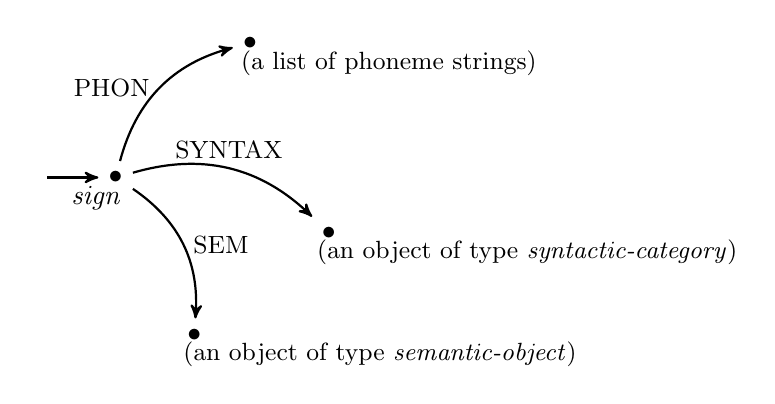
\begin{tikzpicture}[->,>=stealth',auto,node distance=1cm,thick,main node/.style={}]

  \node[main node] (0) {};
  \node[main node] (1) [right of=0] {\ensuremath{\bullet}};
  \node (1t) at (1-.7cm:.8cm) {\textit{sign}};
  \node[main node] (a) [right of=1] {};
  \node[main node] (aa) [above of=a] {};
  \node[main node] (2) [above right of=aa] {\ensuremath{\bullet}};
  \node (2t) at (18:4.7cm) {{\small (a list of phoneme strings)}};
  \node[main node] (b) [right of=a] {};
  \node[main node] (3) [below right of=b] {\ensuremath{\bullet}};
  \node (3t) at (-8.7:6.3cm) {{\small (an object of type \textit{syntactic-category})}};
  \node[main node] (c) [below of=a] {};
  \node[main node] (4) [below of=c] {\ensuremath{\bullet}};
  \node (4t) at (-27.2:4.9cm) {{\small (an object of type \textit{semantic-object})}};


  \path[every node/.style={font=\small}]
    (0) edge node[left] {} (1)
    (1) edge [bend left] node[left] {PHON} (2)
	edge [bend left] node[above] {SYNTAX} (3)
	edge [bend left] node[right] {SEM} (4);
\end{tikzpicture}
\end{document}
